\chapter{Annexe1 - Article JFPC}  
\label{ann_JFPC}
Nous considérerons un problème d'ordonnancement cumulatif dans
lequel les tâches ont une durée et un profil de consommation de
ressource variable. Ce profil, qui peut varier en fonction du temps, est
une variable de décision du problème dont dépend la durée de la tâche
associée. 
Pour ce problème NP-difficle, nous présentons un modèle de programmation
par contraintes et un modèle de programmation linéaire en nombres
entiers (PLNE). De plus, des inégalités valides déduites de la
programmation par contraintes  viennent renforcer le PLNE. 
Ces modèles sont ensuite comparés par le biais d'expérimentations.


\section{Introduction}

Nous étudions un problème d’ordonnancement avec ressource continue et
contraintes énergétiques, le Continuous Energy-Constrained Scheduling
Problem (CECSP). Dans ce problème, un ensemble de tâches ${\cal
A}=\{1,\dots,n\}$ utilisant une ressource continue et cumulative de
capacité limitée $B$ doit être ordonnancé.  La quantité de ressource
nécessaire à l'exécution d'une tâche n'est pas fixée mais - le profil
de consommation de cette dernière est une fonction $b_i(t)$ définie
pour tout  $t \in \mathbb{R}$\footnote{Le domaine de définition de la
fonction peut être réduit mais, pour faciliter les notations, nous
supposons qu'elle est définie pour tout $t \in \mathbb{R}$.} - doit
être déterminé. Une fois la tâche commencée et jusqu'à sa date de fin,
la fonction $b_i(t)$ doit être comprise entre une valeur maximale,
$\bmax$, et minimale, $\bmin$.   

De plus, la consommation, à un instant $t$, d'une partie de
la ressource permet la production d'une certaine quantité d'énergie
et, une tâche finit lorqu'elle a reçu une énergie $W_i$. Cette
énergie est calculée par le biais d'une fonction de rendement $f_i$, 
propre à chaque tâche. Dans cet article, ces fonctions sont supposées
continues, croissantes, affines et peuvent être exprimées de la
manière suivante: 
 
\noindent
  $f_i(b)=\left\{
    \begin{array}{ll} 0 & \quad \text{si }b=0\\ a_i*b+c_i &\quad
                                                            \text{si }\bmin=0\text{ et }b \in ]\bmin,\bmax] \\ a_i*b+c_i &\quad
                                                                                                                           \text{si }\bmin\neq 0 \text{ et }b \in [\bmin,\bmax]
    \end{array} \right.$ 
  
  \noindent
  avec $a_i>0$ et $c_i \geq -a_i*\bmin $ pour
  s'assurer que $f_i(b) \geq 0,\ \forall b \in \inter[\bmin][\bmax]$.

Dans la suite, nous dénotons par $\ES$ et $\LS$
la date de début au plus tôt et au plus tard de $i$ et par
$\EE$ et $\LE$ la date de fin au plus tôt et au
plus tard de $i$.

Pour trouver une solution pour le CECSP, nous devons déterminer, pour
chaque tâche $i \in {\cal A}$, sa date de début $st_i$, sa date de fin
$et_i$ et sa fonction d'allocation de ressource $b_i(t)$, $\forall t
\in {\cal T}=[\min_{i\in{\cal A}} \ES, \max_{i\in {\cal
    A}} \LE]$. De plus, ces variables doivent satisfaire
les contraintes suivantes:
\begin{eqnarray} 
  \ES\le st_i < et_i \le \LE & & \forall i \in
{\cal A} \label {tw_CECSP}\\
  \bmin \le b_i(t) \le \bmax & & \forall i \in {\cal A},\
\forall t \in [st_i,et_i] \label {bminmax_CECSP}\\
  b_i(t)=0 & & \forall i \in {\cal A},\ \forall t \not\in
[st_i,et_i] \label {b0_CECSP}\\
  \int_{st_i}^{et_i} f_i(b_i(t))dt =W_i & & \forall i \in {\cal
A} \label{nrj_CECSP}\\
  \sum_{i \in {\cal A}} b_i(t) \le B & & \forall t \in {\cal
T} \label{res_CECSP}
\end{eqnarray}
L'objectif auquel nous nous sommes intéressés est la minimisation de
la consommation totale de la ressource. Dans~\cite{Nattaf2015}, les
auteurs montrent que trouver une solution admissible pour le CECSP est
déjà un problème NP-complet. 

De plus, une instance ayant des données seulement entières peut
n'avoir que des solutions à valeurs dans
$\mathbb{R}$~\cite{Nattaf2015}. Cependant, une dilatation de
l'instance, i.e. multiplier les données par un certain coefficient
$\alpha$, permet de palier à ce problème. 
De ce fait et dans le but de résoudre des instances entières, nous
nous sommes intéressés, dans un premier temps, à la version discrète
du CECSP, le DECSP (Discrete Energy Constrained Scheduling
Problem). Dans ce problème, toutes les données sont supposées entières
et les domaines de chaque variable ne contiennent
que des valeurs entières, i.e. $st_i,\ et_i,\ b_i(t) \in \mathbb{N}$ et
$b_i(t)$ est défini $\forall t \in {\cal T}_{\cal D}=\{\min_{i\in{\cal
A}} \ES,\dots, \max_{i\in {\cal A}} \LE\}$. 

Pour ce problème, nous présentons un modèle de
programmation par contraintes (PPC) permettant l'utilisation des
algorithmes de propagation mis en place pour la contrainte
cumulative, notamment~\cite{Gay2015}.  Un modèle de
programmation linéaire en nombres entiers (PLNE) est aussi
présenté. Ce modèle est ensuite renforcé à l'aide d'inégalités
valides déduites du raisonnement énergétique~\cite{Lopez1990}. 
Ces deux modèles sont ensuite testés sur des instances à données
entières, avec et sans dilatation.

\section{Modèle de programmation par contrainte}

Pour modéliser le DECSP à l'aide de la PPC, nous divisons chaque tâche
$i$ en deux sous-tâches $i_{min}$ et $i_{preem}$. La première,
$i_{min}$, est une tâche ayant une consommation de ressource fixe,
égale à $\bmin$, et une durée variable $p_i$. Cette tâche
représente la quantité de ressource obligatoirement consommée par une
activité durant son exécution, i.e. $\bmin$.  La seconde, $i_{preem}$
est une tâche préemptive optionnelle, consommant une quantité variable
de ressource comprise entre $0$ et $\bmax-\bmin$ et devant s'exécuter
en même temps que $i_{min}$. Cette tâche est elle-même divisée en
sous-tâches $i_{preem}^\ell,\ \ell \in \{1,\dots, et_i-st_i\}={\cal L}_i$. Notons
que $|{\cal L}_i|=et_i - st_i \le \lceil \frac{W_i}{f_i(\bmin)}\rceil$. 
\begin{ex}
Considérons la tâche possédant les attributs suivant:  $\ES= 0$,
$\LE=6$, $W_i=28$, $r^{min}=1$,
$r^{max}=5$ et $f_i(b)=2b+1$. La Figure~\ref{fig:ex:PPC} présente un
ordonnancement de cette tâche (à droite) et l'ordonnancement
correspondant donné par le modèle (à gauche) avec $r_{i^2_{preem}}=0$. 
\begin{figure}[!htb]
  \centering
  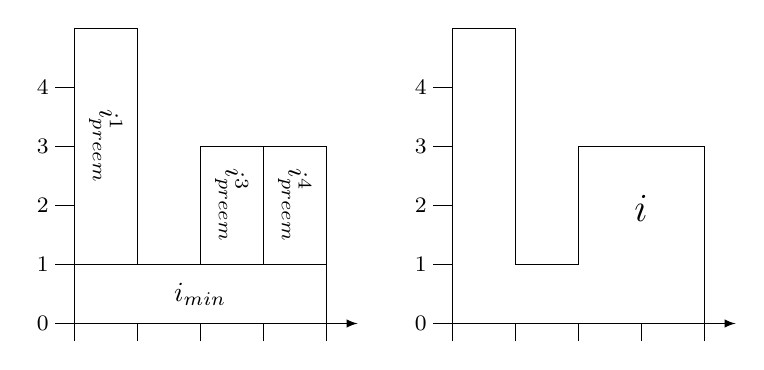
\begin{tikzpicture}
[xscale=0.8,yscale=0.75]
\node (O) at (0,0) {};
\draw (0,0) rectangle (4,1) node[midway] {$i_{min}$};
\draw (0,1) rectangle (1,5) node[midway,rotate=-90] {$i_{preem}^1$};
\draw (2,1) rectangle (3,3) node[midway,rotate=-90] {$i_{preem}^3$};
\draw (3,1) rectangle (4,3) node[midway,rotate=-90] {$i_{preem}^4$};

\draw[->,>=latex] (0,0) -- (4.5,0);

\foreach \i in {0,...,4}
{
  \draw (\i,-0.3) -- (\i,0);
  \draw (-0.3,\i) -- (0,\i)node[left=0.2cm] {\footnotesize \i};
}

\draw (7,5) -- (7,1) -- (8,1) -- (8,3)  -- node[below=0.5cm,midway] {\Large $i$}(10,3)  --  (10,1)
-- (10,0)--  (6,0) -- (6,5) -- cycle;
\draw[->,>=latex] (6,0) -- (10.5,0);

\foreach \i in {0,...,4}
{
  \draw (\i+6,-0.3) -- (\i+6,0);
  \draw (5.7,\i) -- (6,\i) node[left=0.2cm] {\footnotesize \i}; 
}    
  \end{tikzpicture}
  \caption{Exemple de solution du modèle PPC.}
  \label{fig:ex:PPC}
\end{figure}
\end{ex}
Le problème du DECSP peut alors être formulé à l'aide des variables:
\begin{itemize}
\item $i_{min}=\{s_{i_{min}}, e_{i_{min}}, b_{i_{min}},p_{i_{min}}\},\ 
  \forall i \in {\cal A}$ 
\item $i_{preem}^\ell=\{s_{i_{preem}^\ell},e_{i_{preem}^\ell},
  b_{i_{preem}^\ell},p_{i_{preem}^\ell}\}$, $\forall i \in {\cal A},\
  \ell \in {\cal L}_i$.
\end{itemize}
et des contraintes:
\begin{enumerate}  
\item $\forall (i,l) \in {\cal A} \times {\cal L}_i:\
  e_{i_{preem}^\ell} = s_{i_{preem}^{\ell+1}}$ 
\vspace{0.2cm}
\item $\forall i \in {\cal A}:\  s_{i_{min}} = s_{i_{preem}^1}$ et $ e_{i_{preem}^{|{\cal L}_i|}} = e_{i_{min}}$   
\vspace{0.2cm}
\item $\forall t \in  {\cal T}:\\ \sum\limits_{\substack{i \in {\cal A} \\ t \in [s_{i_{min}},e_{i_{min}}[}} b_{i_{min}}
  + \sum\limits_{\substack{(i,l) \in {\cal A}\times {\cal L}_i\\ t \in
      [s_{i_{preem}^\ell},e_{i_{preem}^\ell}[}}
  b_{i_{preem}^\ell} \le B$ 
\vspace{0.2cm}
\item $\forall i \in {\cal A}:\ \sum_{l \in {\cal L}_i} \left(f_i(b_{i_{preem}^\ell})
    (e_{i_{preem}^\ell}-s_{i_{preem}^\ell})\right) +
  f_i(b_{i_{min}}) (e_{i_{min}}-s_{i_{min}}) \ge W_i $
\end{enumerate}
La première contrainte permet d'ordonner les sous-tâches de
$i_{preem}$. Ceci dans le but de faciliter la modélisation des autres
contraintes. La seconde contrainte modélise le fait que $i_{preem}$
commence et finit en même temps que $i_{min}$. La troisième contrainte
assure que la capacité de la ressource n'est pas excédée en sommant, à
un instant $t$, les consommations minimales des tâches en cours ainsi
que les consommations des sous-tâches préemptives en cours. Enfin, la
quatrième contrainte permet de s'assurer que chaque tâche reçoit au
moins l'énergie requise $W_i$. 

Un des avantages de cette formulation est qu'elle permet l'utilisation
des algorithmes de propagation mis en places pour la contrainte
cumulative tels que le time-table classique~\cite{Baptiste2001},
disjonctif~\cite{Gay2015} ou associé au edge-finding~\cite{Vilim2011},
le raisonnement disjonctif~\cite{Baptiste2001}, ou encore le
raisonnement énergétique~\cite{Lopez1990}. Cependant, certains de ces
raisonnements peuvent être adaptés pour 
prendre en compte l'ensemble du problème. C'est le cas, par exemple,
du raisonnement énergétique détaillé ci-dessous.

\subsection{Raisonnement énergétique}


Ce paragraphe présente un algorithme de propagation pour le
DECSP basé sur le raisonnement énergétique défini pour le
CECSP~\cite{Nattaf2015}.  L'adaptation de ce raisonnement au cas
discret est quasi-directe. Cependant, nous rappelons les bases de
celui-ci car nous l'utiliserons dans la suite pour déduire des
inégalités valides pour le PLNE.

Le principe du raisonnement énergétique est de comparer la quantité de
ressource disponible dans un intervalle avec la quantité minimale de
ressource consommée par toutes les tâches dans cet intervalle.

Les configurations pour lesquelles la quantité de ressource requise
par une tâche $i$ dans l'intervalle $[t_1,t_2[$ est minimale
correspondent toujours à une configuration où la tâche reçoit le
maximum d'énergie possible, i.e. est ordonnancée à $\bmax$, en dehors
de $[t_1,t_2[$, tout en respectant les contraintes
\eqref{tw_CECSP}--\eqref{res_CECSP}. Ceci correspond donc à une des
configurations suivantes:
\begin{itemize}
\item la tâche est calée à gauche: ordonnancée à $\bmax$ durant
$[ \ES , t_1 [$;
\item la tâche est calée à droite: ordonnancée à $\bmax$ durant
$[t_2,\LE{[}$;
\item la tâche est centrée: ordonnancée à $\bmax$ durant
$[\ES,t_1[ \cup [t_2,\LE{[}$ ou ordonnancée à
$\bmin$ durant $[t_1,t_2[$.
\end{itemize} En effet, dans le dernier cas, il peut arriver
qu'ordonnancer la tâche à $\bmax$ dans $[\ES,t_1[ \cup
[t_2,\LE{[}$ implique que la quantité d'énergie restant à
apporter à la tâche dans $[t_1,t_2[$ ne soit pas suffisante pour
ordonnancer la tâche à $\bmin$ durant $[t_1,t_2[$. Or, ceci
impliquerait une violation de la
contrainte~\eqref{bminmax_CECSP}. Dans ce cas, la tâche est donc
ordonnancée à $\bmin$ durant l'intervalle $[t_1,t_2[$. Alors la
quantité de ressource requise par la tâche $i$ dans $[t_1,t_2[$ est la
quantité minimale requise par ces configurations.  

Les intervalles $[t_1,t_2[$ sur lesquels appliquer ce test pour le
CECSP sont décrits dans~\cite{Nattaf2015}. Pour le DECSP, nous devons
considérer les projections de ces intervalles sur les entiers,
i.e. $[a,b[ \rightarrow [\lfloor a \rfloor, \lceil b \rceil[$.  Les
ajustements pour le CECSP s'adaptent aussi naturellement au DECSP à
l'aide de cette même projection.

\section{Modèle de programmation linéaire en nombres entiers}
\label{MIP}
\subsection{Modèle}
La formulation proposée dans cet article est une formulation indexée par
le temps. Elle est adaptée de la formulation décrite
dans~\cite{Nattaf2015}. 
Dans ces formulations, l'horizon de temps est divisé en
intervalles de taille 1 et est défini par: ${\cal T}_{\cal D}$. 
Pour chaque activité $i \in {\cal A}$ et pour chaque instant $t \in
{\cal T}_{\cal D}$, nous définissons deux variables binaires $x_{it}$
et $y_{it}$ pour modéliser le début et la fin des activités. La
variable $x_{it}$ (resp. $y_{it}$) prendra la valeur $1$ si et
seulement si l'activité $i$ commence (finit) à l'instant $t$.
Pour modéliser la consommation de ressource et l'apport en énergie,
nous introduisons deux variables, $b_{it}$ et $w_{it}$ qui
représentent respectivement la quantité de
ressource consommée par l'activité $i$ dans la période de temps
$t$ et l'énergie reçue par cette même activité durant cette période. 

Par manque de place, ce modèle n'est pas entièrement décrit ici mais
nous décrivons les contraintes permettant de lier les variables
$b_{it}$ et $w_{it}$, i.e. permettant de calculer l'énergie apportée à
$i$ dans la période $t$, $w_{it}$ , en fonction de la consommation de
ressource $b_{it}$. Nous donnons aussi le nombre de variables et de
contraintes du modèle.

Les contraintes liant $b_{it}$ et $w_{it}$, $\quad \forall t\in {\cal T}_{\cal D},\
\forall i \in {\cal A}$ sont les suivantes:
\begin{equation}  w_{it}=a_ib_{it}+c_i\left(\sum_{\tau=\ES}^t
x_{i\tau}-\sum_{\tau=\ES+1}^t y_{i\tau}\right)  \label{conv_CECSP_TI}
\end{equation} Cette contrainte nous permet de modéliser la fonction
de rendement $f_i,\ \forall i \in {\cal A}$. En effet,
$\left(\sum_{\tau=\ES}^t x_{i\tau}-\sum_{\tau=\ES+1}^t
y_{i\tau}\right) $ est égale à $1$ si et seulement si l'activité $i$
est en cours à l'instant $t$.  Dans ce cas là, la valeur de l'énergie
apportée à $i$ est bien $w_{it}=a_ib_{it}+c_i$. Le second cas se
produit quand l'activité $i$ n'est pas en cours à $t$. Dans ce cas,
$b_{it}=0$ implique $w_{it}=0$.

Le modèle possède donc $2n|{\cal T}_{\cal D}|$ variables binaires,
$2n|{\cal T}_{\cal D}|$ variables continues et au plus $3n+|{\cal
T}_{\cal D}|*(6n+1)$ contraintes.

\section{Inégalités valides basées sur le raisonnement énergétique}
Ce paragraphe décrit des inégalités valides déduites du raisonnement
énergétique pour le PLNE. Soit ${\cal R}$ l'ensemble des intervalles
d'intérêt pour le raisonnement énergétique.
\begin{align}
&(x_{i\ES} + y_{i\LE} -1 ) \, \bb + \sum_{j\neq i}
  \bb[j] \le \nonumber\\ 
&  B(t_2-t_1) \quad \forall i \in {\cal A},\ \forall
  [t_1,t_2] \in {\cal R}
\label{both}\\[2mm] 
&(x_{i\ES} + \sum_{t=t_1}^{t_2}y_{it} -1) \, \bb + \sum_{j\neq i}
  \bb[j] \le \nonumber \\
&  B(t_2-t_1) \quad \forall i \in {\cal A},\ \forall
  [t_1,t_2] \in {\cal R}
\label{left}\\[2mm] 
&(\sum_{t=t_1}^{t_2}x_{it} + y_{i\LE}-1) \, \bb + \sum_{j\neq i}
  \bb[j] \le \nonumber\\
&  B(t_2-t_1) \quad \forall i \in {\cal A},\ \forall
  [t_1,t_2] \in {\cal R}
\label{right}\\[2mm] 
&(1-\sum_{t<t_1}x_{it} - \sum_{t>t_2}y_{it}) \, \bb + \sum_{j\neq i}
  \bb[j] \le \nonumber \\
&  B(t_2-t_1) \quad \forall i \in {\cal A},\ \forall
  [t_1,t_2] \in {\cal R}
\label{total}\\[2mm] 
&(\sum_{t\le t_1}x_{it} + \sum_{t\ge t_2}y_{it} -1 ) \, \bb  \le
B(t_2-t_1) \nonumber\\
&\forall i \in {\cal A},\ \forall
[t_1,t_2] \in {\cal R}
\label{min}
\end{align}

L'inégalité~\eqref{both} correspond au cas où la tâche est centrée et est
ordonnancée à $\bmax$ durant $[\ES,t_1] \cup
[t_2,\LE{]}$. En effet, cette inégalité n'est active que dans
le cas où $(x_{i\ES} + y_{i\LE} -1 )= 1 \Rightarrow
\left[x_{i\ES}=1\land y_{i\LE}=1\right]$. Or,
ceci implique que la tâche commence à $\ES$ et finit
$\LE$. Donc, la ressource disponible dans $[t_1,t_2[$ doit
être suffisante pour donner la quantité de ressource minimale requise
par $i$ dans $[t_1,t_2[$ dans cette configuration.  Dans tous les
autres cas, l'inégalité devient $\sum_{j\neq i} \bb[j] \le B(t_2-t_1)$
ou $\sum_{j\neq i} \bb[j] - \bb \le B(t_2-t_1)$.

Les inégalités \eqref{left}, \eqref{right}, \eqref{total}, \eqref{min}
correspondent respectivement au cas où $i$ est calée à gauche, $i$ est
calée à droite, $i$ est complètement incluse dans $[t_1,t_2]$, $i$ est
exécutée à $\bmin$ durant l'intervalle $[t_1,t_2]$ et sont déduites de
la même façon que~\eqref{both}.  Ces inégalités seront ajoutées au
modèle indexé par le temps décrit à la section~\ref{MIP} pour
renforcer ce dernier. 
 
\section{Résultats Expérimentaux}

Nous avons testé les différentes méthodes de résolution proposées dans
cet article sur les instances de~\cite{Nattaf2015}. Les
expérimentations ont été conduites sous le système d'exploitation
Ubuntu 64-bit 12.04 et les résultats sont calculés au moyen d'un
processeur 4-core, 8 thread Core (TM) i7-4770 CPU et de 8GB de mémoire
RAM. 

Le modèle de PLNE est résolu à l'aide de IBM Cplex 12.6 avec 2 threads
et une limite de temps de 100 secondes. Les inégalités déduites du
raisonnement énergétique sont calculées avant la résolution du PLNE et
ajoutées statiquement au modèle. Ceci augmente la taille du modèle de
$5|{\cal R}|n$ contraintes (avec $|{\cal R}| \in O(n^2)$). 

Le tableau~\ref{table1} décrit les résultats du PLNE. 

L'ajout des inégalités du raisonnement énergétique permet de résoudre
les instances à $25$ tâches de manières plus efficace. Cependant, elles
ralentissent le modèle pour les instances à $20$ ou $30$ tâches mais
la perte de rapidité dans ce cas là est beaucoup moins élevée que le
gain fait sur les instances à $25$. Une poursuite de recherche
intéressante serait d'essayer d'ajouter ces contraintes pendant la
résolution du PLNE en tant que coupes. 

Le modèle de PPC est résolu avec IBM CP Optimizer 12.6. Le
tableau~\ref{table2} décrit les résultats du modèle de PPC.  Le modèle 
de PPC est testé sans ajout du raisonnement énergétique présentés dans
cet article mais le modèle utilise les propagateurs du solveur. Des
résultats expérimentaux plus détaillées seront proposés lors de la
conférence.
\begin{table}
\centering
    \begin{tabular}{|c|c|cc|cc|}
      \hline
       & & \multicolumn{2}{c|}{$1^{ère}$ sol.} & \multicolumn{2}{c|}{fin algo.}\\
      \hline
    &  \#tâches & temps(s) &  écart & temps  & \%opt. \\
      \hline
      DEF	&	20	&	5.37	&	7.85	&	75.4	&	0.25\\
      ER	&	20	&	8.4	&	10.6	&	78.9	&	0.22\\
      \hline
      DEF	&	25	&	4.6	&	4.4	&	83.8	&	0.17\\
      ER	&	25	&	0.06	&	3.86	&	60.1	&	0.4\\
      \hline
      DEF	&	30	&	0.99	&	7.18	&	75.19	&	0.25\\
      ER	&	30	&	5.66	&	7.53	&	75.8	&	0.25\\
      \hline
    \end{tabular}
  \caption{Résultats du PLNE avec et sans inégalités valides: ER et
    DEF resp. (TL 1000s)}
  \label{table1}
\end{table}


\begin{table}
\centering
    \begin{tabular}{|c|cc|cc|}
      \hline
      & \multicolumn{2}{c|}{$1^{ère}$ sol.} & \multicolumn{2}{c|}{fin algo.}\\
      \hline
      \#tasks & time & deviation & time lim. &  \%solved \\
      \hline
20	&0.19&	34.1&	100&	95\\
25	&0.3	&47.9&	100	&91\\
30	&0.42	&43.1	&100	&95\\
      \hline
    \end{tabular}
  \caption{Résultats du modèle PPC}
\label{table2}
\end{table}

Les résultats montrent l'intérêt des inégalités valides ajoutées au
PLNE. Le modèle de PPC ne permet pas de prouver l'optimalité des solutions
trouvées mais a des résultats similaires au PLNE. En effet, dans
presque tous les cas, le modèle de PPC trouve une solution aussi bonne
que le PLNE, sans toutefois prouver son optimalité.

Les méthodes présentées ont aussi été testées sur des instances
dilatées dans le but de garantir l'existence de solutions entières.  
La dilatation est effectuée de la manière suivante. Soit $\alpha$ le
plus petit commun 
multiple à tous les $\bmin$ et $\bmax$. Alors, la dilatation
consiste à multiplier $\LE,\ \EE,\
\LS,\ \ES$ et $W_i$ par $\alpha$. Ces
expérimentations n'ont pas donné de résultats dû à la grande taille
de ces modèles. Les modèles continus pourraient donc rester  la
seule alternative pour obtenir des solutions optimales dans le cas où
la solution est réelle.

Parmi les poursuites de recherche possibles, on trouve l'amélioration
des modèles avec la réduction du nombre de variable et/ou de contraintes et la
mise en place d'algorithmes de propagation dédiés.
\newpage
\begin{bibunit}[alpha]
\nocite{JFPC}
\nocite*
\putbib[JFPC]
\end{bibunit}







